\label{cha:performance_protein}
The following chapter is dedicated to evaluate the different machine learning and feature engineering methods on
the target compounds. For each protein the top two approaches are evaluated further.

\subsection{Acetylcholinesterase}
The following table presents the results of the different machine learning algorithms on the various
test-sets. The ROC curves for the top two performing configurations can be found at \ref{fig:ache_baseline_rf_roc} and \ref{fig:ache_smote_rf_roc}
respectively. The confusion matrices can be found at \ref{fig:ache_baseline_rf_conf} and \ref{fig:ache_smote_rf_conf}.
The scoring functions achieved an accuracy score of 81.06\% on the test-set.
\begin{table}[H]
    \begin{center}
        \caption{Acetylcholinesterase performance test-set}
        \begin{tabular}{lrrrrr}
            \toprule
            Name             & ACC    & FPR    & AUC    & EF     & REF     \\
            \midrule
            baseline\_rf     & 0.8106 & 0.3285 & 0.7992 & 1.4161 & 92.6829 \\
            fe\_smote\_rf    & 0.8007 & 0.3358 & 0.7894 & 1.4046 & 91.4634 \\
            fe\_smote\_nn    & 0.7708 & 0.2993 & 0.7650 & 1.4102 & 82.9268 \\
            baseline\_nn     & 0.7674 & 0.2920 & 0.7626 & 1.4134 & 81.7073 \\
            fe\_rf\_per\_knn & 0.7575 & 0.4307 & 0.7420 & 1.3172 & 91.4634 \\
            baseline\_knn    & 0.6844 & 0.5766 & 0.6629 & 1.1966 & 90.2439 \\
            fe\_rf\_mdi\_knn & 0.5515 & 0.4307 & 0.5530 & 1.0987 & 59.8639 \\
            \bottomrule
        \end{tabular}
    \end{center}
\end{table}

\begin{figure}[H]
    \begin{center}
        \caption[]{Baseline random forest confusion matrix}
        \label{fig:ache_baseline_rf_conf}
        \includegraphics[height=9cm]{ache/baseline_rf_conf.jpg}
    \end{center}
\end{figure}

\begin{figure}[H]
    \begin{center}
        \caption[]{SMOTE random forest confusion matrix}
        \label{fig:ache_smote_rf_conf}
        \includegraphics[height=9cm]{ache/fe_smote_rf_conf.jpg}
    \end{center}

\end{figure}

\begin{figure}[H]
    \begin{center}
        \caption[]{Baseline random forest ROC curve}
        \label{fig:ache_baseline_rf_roc}
        \includegraphics[height=9cm]{ache/baseline_rf_roc.jpg}
    \end{center}

\end{figure}

\begin{figure}[H]
    \begin{center}
        \caption[]{SMOTE random forest ROC curve}
        \label{fig:ache_smote_rf_roc}
        \includegraphics[height=9cm]{ache/fe_smote_rf_roc.jpg}
    \end{center}
\end{figure}


\subsection{Cyclooxygenase 1}
The following table presents the results of the different machine learning algorithms on the various
test-sets. The ROC curves for the top two performing configurations can be found at \ref{fig:cox1_baseline_rf_roc} and \ref{fig:cox1_smote_rf_roc}
respectively. The confusion matrices can be found at \ref{fig:cox1_baseline_rf_conf} and \ref{fig:cox1_smote_rf_conf}.
The scoring functions achieved an accuracy score of 77.24\% on the test-set.

\begin{table}[H]
    \begin{center}
        \caption{Cyclooxygenase 1 performance test-set}
        \begin{tabular}{lrrrrr}
            \toprule
            Name             & ACC    & FPR    & AUC    & EF     & REF     \\
            \midrule
            baseline\_rf     & 0.7724 & 0.0183 & 0.6344 & 2.8909 & 87.0968 \\
            fe\_smote\_rf    & 0.7628 & 0.0138 & 0.6155 & 2.9362 & 88.4615 \\
            fe\_rf\_per\_knn & 0.7019 & 0.0826 & 0.5598 & 1.7044 & 51.3514 \\
            baseline\_knn    & 0.6859 & 0.1147 & 0.5544 & 1.5153 & 45.6522 \\
            baseline\_nn     & 0.6827 & 0.0872 & 0.5309 & 1.4081 & 42.4242 \\
            fe\_smote\_nn    & 0.6827 & 0.1147 & 0.5490 & 1.4752 & 44.4444 \\
            fe\_rf\_mdi\_knn & 0.6250 & 0.1835 & 0.4987 & 0.9899 & 29.8246 \\
            \bottomrule
        \end{tabular}
    \end{center}
\end{table}

\begin{figure}[H]
    \begin{center}
        \caption[]{Baseline random forest confusion matrix}
        \label{fig:cox1_baseline_rf_conf}
        \includegraphics[height=9cm]{cox1/baseline_rf_conf.jpg}
    \end{center}
\end{figure}

\begin{figure}[H]
    \begin{center}
        \caption[]{SMOTE random forest confusion matrix}
        \label{fig:cox1_smote_rf_conf}
        \includegraphics[height=9cm]{cox1/fe_smote_rf_conf.jpg}
    \end{center}

\end{figure}

\begin{figure}[H]
    \begin{center}
        \caption[]{Baseline random forest ROC curve}
        \label{fig:cox1_baseline_rf_roc}
        \includegraphics[height=9cm]{cox1/baseline_rf_roc.jpg}
    \end{center}

\end{figure}

\begin{figure}[H]
    \begin{center}
        \caption[]{SMOTE random forest ROC curve}
        \label{fig:cox1_smote_rf_roc}
        \includegraphics[height=9cm]{cox1/fe_smote_rf_roc.jpg}
    \end{center}
\end{figure}

\subsection{Dipeptidyl peptidase IV}
The following table presents the results of the different machine learning algorithms on the various
test-sets. The ROC curves for the top two performing configurations can be found at \ref{fig:dpp4_baseline_rf_roc} and \ref{fig:dpp4_smote_rf_roc}
respectively. The confusion matrices can be found at \ref{fig:dpp4_baseline_rf_conf} and \ref{fig:dpp4_smote_rf_conf}.
The scoring functions achieved an accuracy score of 77.21\% on the test-set.

\begin{table}[H]
    \begin{center}
        \caption{Dipeptidyl peptidase IV performance test-set}
        \begin{tabular}{lrrrrr}
            \toprule
            Name             & ACC    & FPR    & AUC    & EF     & REF     \\
            \midrule
            baseline\_rf     & 0.7721 & 0.2041 & 0.7730 & 1.5393 & 79.8387 \\
            fe\_smote\_rf    & 0.7662 & 0.2122 & 0.7670 & 1.5254 & 79.1165 \\
            fe\_rf\_per\_knn & 0.7112 & 0.3714 & 0.7082 & 1.3412 & 78.7879 \\
            baseline\_nn     & 0.6896 & 0.3347 & 0.6887 & 1.3425 & 71.2121 \\
            baseline\_knn    & 0.6896 & 0.3959 & 0.6865 & 1.3046 & 76.8939 \\
            fe\_smote\_nn    & 0.6896 & 0.3306 & 0.6889 & 1.3453 & 70.8333 \\
            fe\_rf\_mdi\_knn & 0.4892 & 0.5143 & 0.4891 & 0.9791 & 50.7812 \\
            \bottomrule
        \end{tabular}
    \end{center}
\end{table}

\begin{figure}[H]
    \begin{center}
        \caption[]{Baseline random forest confusion matrix}
        \label{fig:dpp4_baseline_rf_conf}
        \includegraphics[height=9cm]{dpp4/baseline_rf_conf.jpg}
    \end{center}
\end{figure}

\begin{figure}[H]
    \begin{center}
        \caption[]{SMOTE random forest confusion matrix}
        \label{fig:dpp4_smote_rf_conf}
        \includegraphics[height=9cm]{dpp4/fe_smote_rf_conf.jpg}
    \end{center}

\end{figure}

\begin{figure}[H]
    \begin{center}
        \caption[]{Baseline random forest ROC curve}
        \label{fig:dpp4_baseline_rf_roc}
        \includegraphics[height=9cm]{dpp4/baseline_rf_roc.jpg}
    \end{center}

\end{figure}

\begin{figure}[H]
    \begin{center}
        \caption[]{SMOTE random forest ROC curve}
        \label{fig:dpp4_smote_rf_roc}
        \includegraphics[height=9cm]{dpp4/fe_smote_rf_roc.jpg}
    \end{center}
\end{figure}
\subsection{Monoamine oxidase B}
The following table presents the results of the different machine learning algorithms on the various
test-sets. The ROC curves for the top two performing configurations can be found at \ref{fig:maob_baseline_rf_roc} and \ref{fig:maob_fe_rf_per_knn_roc}
respectively. The confusion matrices can be found at \ref{fig:maob_baseline_rf_conf} and \ref{fig:maob_fe_rf_per_knn_conf}.
The scoring functions achieved an accuracy score of 75.98\% on the test-set.

\begin{table}[H]
    \begin{center}
        \caption{Monoamine oxidase B performance test-set}
        \begin{tabular}{lrrrrr}
            \toprule
            Name             & ACC    & FPR    & AUC    & EF     & REF     \\
            \midrule
            baseline\_rf     & 0.7589 & 0.1389 & 0.7181 & 1.9515 & 69.6970 \\
            fe\_rf\_per\_knn & 0.7054 & 0.1944 & 0.6653 & 1.6800 & 60.0000 \\
            fe\_smote\_rf    & 0.7054 & 0.1944 & 0.6653 & 1.6800 & 60.0000 \\
            baseline\_nn     & 0.6964 & 0.1806 & 0.6472 & 1.6625 & 59.3750 \\
            baseline\_knn    & 0.6786 & 0.1667 & 0.6167 & 1.6000 & 57.1429 \\
            fe\_smote\_nn    & 0.6696 & 0.2222 & 0.6264 & 1.5200 & 54.2857 \\
            fe\_rf\_mdi\_knn & 0.5804 & 0.3333 & 0.5458 & 1.1610 & 42.5000 \\
            \bottomrule
        \end{tabular}
    \end{center}
\end{table}

\begin{figure}[H]
    \begin{center}
        \caption[]{Baseline random forest confusion matrix}
        \label{fig:maob_baseline_rf_conf}
        \includegraphics[height=9cm]{maob/baseline_rf_conf.jpg}
    \end{center}
\end{figure}

\begin{figure}[H]
    \begin{center}
        \caption[]{Feature engineering permutation importance confusion matrix}
        \label{fig:maob_fe_rf_per_knn_conf}
        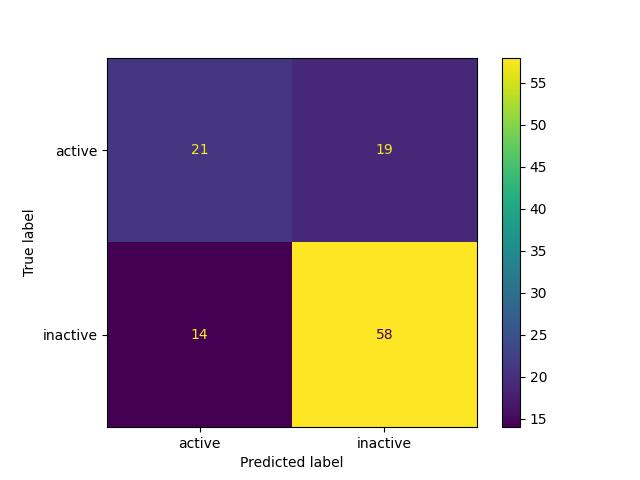
\includegraphics[height=9cm]{maob/fe_rf_per_knn_conf.jpg}
    \end{center}

\end{figure}

\begin{figure}[H]
    \begin{center}
        \caption[]{Baseline random forest ROC curve}
        \label{fig:maob_baseline_rf_roc}
        \includegraphics[height=9cm]{maob/baseline_rf_roc.jpg}
    \end{center}

\end{figure}

\begin{figure}[H]
    \begin{center}
        \caption[]{Feature engineering permutation importance ROC curve}
        \label{fig:maob_fe_rf_per_knn_roc}
        \includegraphics[height=9cm]{maob/fe_rf_per_knn_roc.jpg}
    \end{center}
\end{figure}

\subsection{Soluble epoxide hydrolase}
The following table presents the results of the different machine learning algorithms on the various
test-sets. The ROC curves for the top two performing configurations can be found at \ref{fig:seh_fe_rf_per_knn_roc} and \ref{fig:seh_baseline_nn_roc}
respectively. The confusion matrices can be found at \ref{fig:seh_fe_rf_per_knn_conf} and \ref{fig:seh_baseline_nn_conf}.
The scoring functions achieved an accuracy score of 80.00\% on the test-set.

\begin{table}[H]
    \begin{center}
        \caption{Soluble epoxide hydrolase performance test-set}
        \begin{tabular}{lrrrrr}
            \toprule
            Name             & ACC    & FPR    & AUC    & EF     & REF      \\
            \midrule
            fe\_rf\_per\_knn & 0.8000 & 0.0667 & 0.6667 & 2.6667 & 66.6667  \\
            baseline\_nn     & 0.7833 & 0.0667 & 0.6333 & 2.5000 & 62.5000  \\
            baseline\_rf     & 0.7667 & 0.0000 & 0.5333 & 4.0000 & 100.0000 \\
            fe\_smote\_rf    & 0.7667 & 0.0000 & 0.5333 & 4.0000 & 100.0000 \\
            baseline\_knn    & 0.7333 & 0.0222 & 0.4889 & 0.0000 & 0.0000   \\
            fe\_rf\_mdi\_knn & 0.7000 & 0.1333 & 0.5333 & 1.3333 & 33.3333  \\
            fe\_smote\_nn    & 0.7000 & 0.0889 & 0.4889 & 0.8000 & 20.0000  \\
            \bottomrule
        \end{tabular}
    \end{center}
\end{table}

\begin{figure}[H]
    \begin{center}
        \caption[]{Feature engineering permutation importance confusion matrix}
        \label{fig:seh_fe_rf_per_knn_conf}
        \includegraphics[height=9cm]{seh/fe_rf_per_knn_roc.jpg}
    \end{center}
\end{figure}

\begin{figure}[H]
    \begin{center}
        \caption[]{Baseline neural network confusion matrix}
        \label{fig:seh_baseline_nn_conf}
        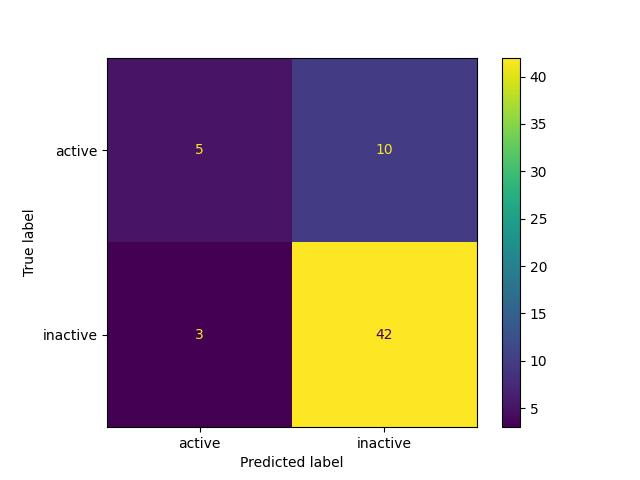
\includegraphics[height=9cm]{seh/baseline_nn_conf.jpg}
    \end{center}

\end{figure}

\begin{figure}[H]
    \begin{center}
        \caption[]{Feature engineering permutation importance ROC curve}
        \label{fig:seh_fe_rf_per_knn_roc}
        \includegraphics[height=9cm]{seh/fe_rf_per_knn_roc.jpg}
    \end{center}

\end{figure}

\begin{figure}[H]
    \begin{center}
        \caption[]{Baseline neural network ROC curve}
        \label{fig:seh_baseline_nn_roc}
        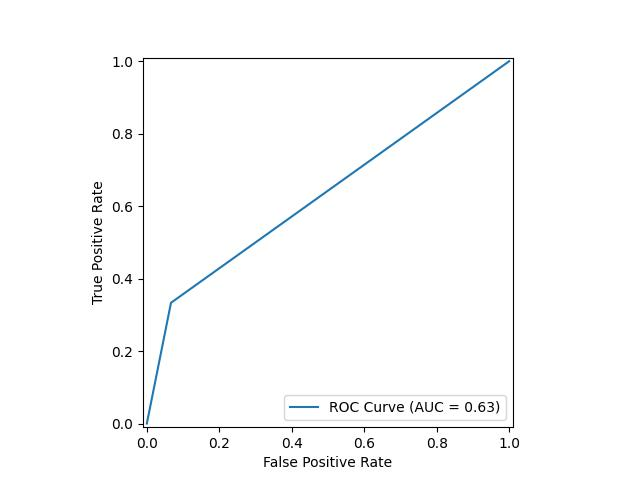
\includegraphics[height=9cm]{seh/baseline_nn_roc.jpg}
    \end{center}
\end{figure}